\documentclass[border=2pt]{standalone}
\usepackage{tikz}
\usetikzlibrary{arrows.meta,positioning,fit,calc}
\begin{document}
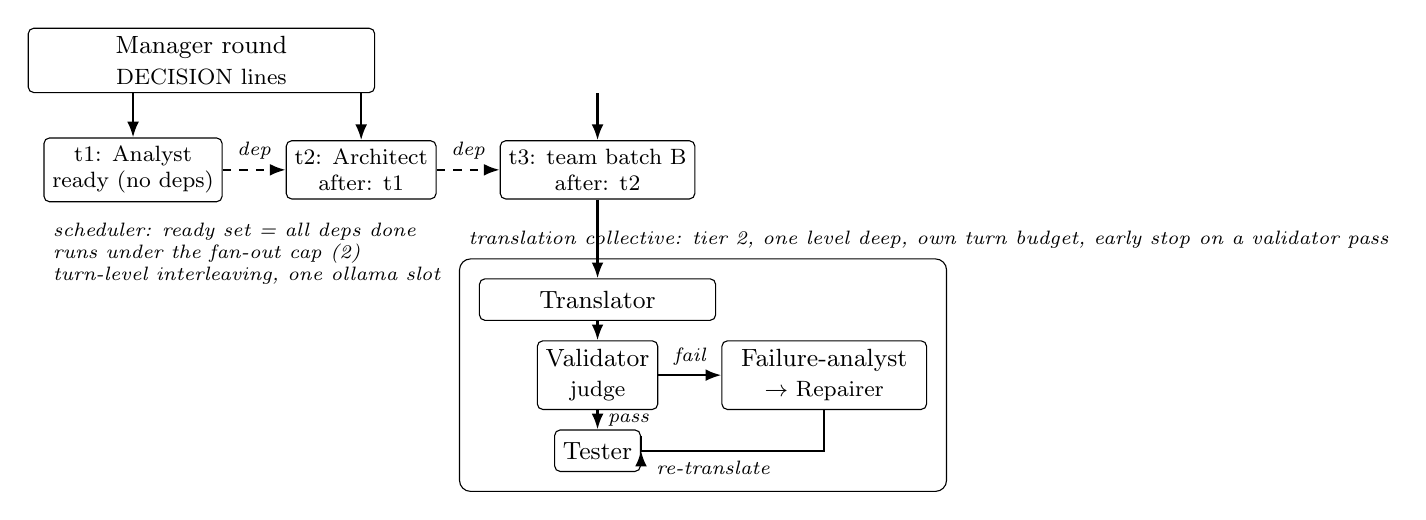
\begin{tikzpicture}[
  font=\small,
  role/.style={draw, rounded corners=2pt, align=center, inner sep=3pt, minimum height=1.5em},
  task/.style={draw, rounded corners=2pt, align=center, inner sep=3pt, font=\footnotesize, minimum height=1.5em},
  cont/.style={draw, rounded corners=4pt, inner sep=7pt},
  arr/.style={-{Latex[length=2mm]}, thick},
  lab/.style={font=\scriptsize\itshape}
]

% Manager round
\node[role, minimum width=44mm] (manager) {Manager round\\ \footnotesize DECISION lines};

% Three delegations
\node[task, below=16pt of manager.south west, anchor=north west, xshift=2mm] (t1) {t1: Analyst\\ \footnotesize ready (no deps)};
\node[task, right=8mm of t1] (t2) {t2: Architect\\ \footnotesize after: t1};
\node[task, right=8mm of t2] (t3) {t3: team batch B\\ \footnotesize after: t2};

\draw[arr] (manager.south -| t1.north) -- (t1.north);
\draw[arr] (manager.south -| t2.north) -- (t2.north);
\draw[arr] (manager.south -| t3.north) -- (t3.north);

% Dependency edges between tasks
\draw[arr, dashed] (t1.east) -- node[lab, above]{dep} (t2.west);
\draw[arr, dashed] (t2.east) -- node[lab, above]{dep} (t3.west);

% Ready-set scheduling note
\node[lab, below=4pt of t1.south west, anchor=north west, align=left] (sched) {scheduler: ready set = all deps done\\runs under the fan-out cap (2)\\turn-level interleaving, one ollama slot};

% Collective nested under t3
\node[role, below=10mm of t3.south, anchor=north, minimum width=30mm] (translator) {Translator};
\node[role, below=7pt of translator] (validator) {Validator\\ \footnotesize judge};
\node[role, below=7pt of validator] (tester) {Tester};
\node[role, right=8mm of validator, minimum width=26mm] (repair) {Failure-analyst\\ \footnotesize $\rightarrow$ Repairer};

\draw[arr] (t3.south) -- (translator.north);
\draw[arr] (translator) -- (validator);
\draw[arr] (validator) -- node[lab, right]{pass} (tester);

% repair loop
\draw[arr] (validator.east) -- node[lab, above]{fail} (repair.west);
\draw[arr] (repair.south) |- ($(tester.east)+(3pt,0)$) -| node[lab, pos=0.2, below right]{re-translate} (tester.east);

% collective container
\node[cont, fit=(translator)(validator)(tester)(repair)] (collbox) {};
\node[lab, anchor=south west] at (collbox.north west)
  {translation collective: tier 2, one level deep, own turn budget, early stop on a validator pass};

\end{tikzpicture}
\end{document}
